\icode{E-MK-MU-L3-260625-003}
如图所示，光滑的斜面上有\(A\)、\(B\)、\(C\)、\(D\)、\(E\)五个点，彼此之间的距离均相等，一小球以某一初速度从\(E\)点滑上斜面做匀减速直线运动，运动到\(A\)点小球速度恰好为零，则下列说法正确的是\paren[CD]

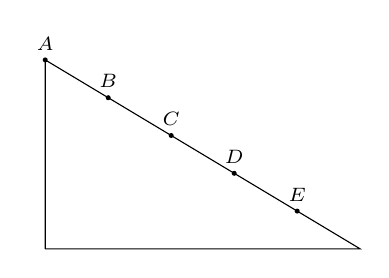
\begin{tikzpicture}[scale=.8,font=\scriptsize]
    \draw (0,0)--(0,3)--(5,0)--(0,0);
    \foreach \y/\c/\x in {3/A/0,2.4/B/1,1.8/C/2,1.2/D/3,.6/E/4}
        \fill (\x,\y)node[above]{\(\c\)} circle(.04);
\end{tikzpicture}
\begin{choices}
    \item 小球经过各点的速度关系为\(v_B - v_A = v_C - v_B\)
    \item \(C\)点的速度与\(E\)点的速度关系为\(v_C = \frac{v_E}{2}\)
    \item 小球从\(E\)点到\(A\)点的平均速度等于\(B\)点的速度
    \item 小球从\(E\)点到\(C\)点的时间小于从\(C\)点到\(A\)点的时间
\end{choices}
\begin{answer}
    CD
\end{answer}